% Korean translation of the v2 manuscript. Same structure, same figures, same
% bibliography keys as main.tex. Compile with: xelatex main_ko.tex (twice).
\documentclass[journal]{IEEEtran}
\usepackage{cite}
\usepackage{amsmath,amssymb,amsfonts}
\usepackage{graphicx}
\usepackage{textcomp}
\usepackage{xcolor}
\usepackage{booktabs}
\usepackage{url}
\usepackage{hyperref}
\usepackage{tabularx}
\usepackage{multirow}
\usepackage{float}
\usepackage{fontspec}
\usepackage{kotex}

\begin{document}

\title{KOSHA-Braille: 한국 화학 안전 정보의 인프라급 접근성}

\author{김유용
\thanks{원고 제출 2026년 4월.}
\thanks{김유용은 위스콘신--매디슨 대학교 소속이다 (e-mail: ykim288@wisc.edu).}
\thanks{ORCID: 0009-0006-4842-666X}
}

\markboth{IEEE Access, VOL. XX, NO. X, 2026}
{Kim: KOSHA-Braille (Korean)}

\begin{abstract}
\textbf{목적.} 한국의 화학 안전 정보는 오직 시각 문서로만 생산되어, 시각장애인이 화학 인접 직역(연구, 규제, 노동 옹호, 공직)에 진입하는 것을 사실상 봉쇄해 왔다. 본 논문은 한국 물질안전보건자료(MSDS) 점자 코퍼스의 구축·검증·공개 릴리스를 보고하며, 이를 사용성(usability) 산출물이 아니라 UN 장애인권리협약 제9조 및 한국 장애인차별금지법 제21조에 근거한 접근성 \emph{인프라}로 위치 짓는다.

\textbf{방법.} 우리는 2017년 한국 점자 규정을 충실히 구현한 결정론적 한국어 점자 인코더를 설계하고, 이를 공공데이터포털을 통해 접근한 KOSHA MSDS 데이터베이스 전체에 적용하였다. 산출물은 독립적으로 개발된 오픈소스 한국어 점자 변환기와 교차 검증되었다. 코퍼스, 인코더, 디코더, 평가 하네스, 그리고 참조 웹 배포는 모두 오픈 소스로 공개되며, 본 논문의 모든 수치적 주장은 릴리스에 동봉된 검증 스크립트로 재생성된다.

\textbf{결과.} 공개 산출물은 48{,}966종의 화학물질, 769{,}897행의 원본 섹션 데이터베이스(이 중 401{,}272개 섹션이 실질적인 한국어 본문을 보유)를 포괄하며, 총 약 1억 1{,}930만 한국어 문자 및 2억 3{,}230만 점자 셀에 이른다. 인코더는 독립 참조 구현과 442건의 교차 검증 사례에서 100\% 일치하였고, 공개 한국어 라운드트립 골든 셋은 45/45로 회복되었다.

\textbf{결론.} 본 연구의 기여는 그간 미공급 상태로 방치되어 온 규제 정보 영역에 대한 인프라급 접근성 릴리스이다. 시각장애 독자를 대상으로 한 읽기 이해 사용자 연구는 필수 후속 작업으로 명시하고 본 제출의 범위에서 의도적으로 분리하였다. 본 논문은 설계·구현·공개 릴리스 연구로 명확히 위치 지어지며, 최종 사용자 평가 연구가 아니다.
\end{abstract}

\begin{keywords}
접근성 인프라, 점자, 한국 점자, 화학 안전 정보, MSDS 데이터셋, 장애인 권리.
\end{keywords}

\titlepgskip=-15pt

\maketitle

\section{서론}
\label{sec:introduction}

\subsection{서비스가 아닌 인프라로서의 접근성}

공공 접근성 시스템---점자블록, 스크린도어, 방송 음성해설, 국회 진행에 대한 수어 통역---은 한 가지 구조적 속성을 공유한다. 이들의 정당성은 일일 사용량에 좌우되지 않는다. 이들은 인프라이다. 그 기능은 장애인의 참여가 \emph{비로소 가능해지는 조건} 자체를 마련하는 데 있다. 이런 시스템을 시장형 수요 지표로 평가하는 것은 \emph{서비스}(재량적·탄력적)와 \emph{인프라}(기초적·비탄력적)를 혼동하는 것이며, 발생 빈도는 낮지만 결과가 중대한 접근(low-incidence, high-stakes access)을 체계적으로 과소평가한다.

본 논문은 이 관점을 격차가 특히 두드러지는 한 영역, 곧 한국 규제 체계 하의 화학 안전 정보에 적용한다. 물질안전보건자료(MSDS, 국제적으로는 SDS)는 유해성 분류, 안전 취급 절차, 비상 조치, 노출 한계 정보를 담은 의무 문서이다 \cite{kosha_act}. 이는 화학자, 산업위생사, 응급대응 인력, 산업안전감독관, 산업재해 피해자 변호사, 기자, 국회의원, 노동조합 조직가 등이 읽는다. 한국에서 이 문서들은 산업안전보건법 \cite{kosha_act}에 따라 시각 문서로만 생산되며, 따라서 점자 사용자에게는 접근 불가능한 상태로 남는다.

\subsection{자기충족적 배제 문제}

영역 특화 점자 인프라 생산에 대한 가장 흔한 반론은 예상 사용자 수가 적다는 것이다. 한국 화학 안전 영역에 한정하면, 관측되는 시각장애 화학자·화학공학자·화학안전규제자는 사실상 0에 가깝다. 우리는 이 관측이 인프라에 반(反)하는 증거가 아니라 오히려 인프라에 \emph{찬성}하는 증거라고 본다. 직역 내 낮은 관측 참여율은 접근 불가능한 직무 정보의 예측 가능한 결과이지, 선호나 능력에 관한 독립적 사실이 아니다.

화학 인접 영역에서 시각장애인이 인프라가 마련된 곳에서 실제로 참여한 선례는 존재한다. 헨리 ``호비'' 웨들러는 2016년 캘리포니아대학교 데이비스 캠퍼스에서 3D 프린팅 분자 모형 보조 장치를 활용해 계산화학 분야 박사학위를 취득하였고, 이후 Accessible Science를 설립하여 시각장애 학생을 위한 화학 교육을 확장하였다 \cite{wedler}. 여러 관할권에서는 시각장애인이 기술 분야 입법 업무를 수행하고 \cite{nfb_legislators}, 장애인 권리 단체는 화학 노출 소송과 규제 옹호 활동을 수행해 왔다. 이러한 사례들은 능력과 관심이 존재함을 보여 주며, 한국의 경우 부재한 것은 다름 아닌 읽기 인프라이다.

상황은 화학자가 아니지만 직무상 MSDS를 반드시 읽어야 하는 2차 독자에 의해 더욱 분명해진다. 산업통상자원부 장관 질의서를 준비하는 보좌진, 산업재해를 기록하는 노동감독관, 직업병 소송을 진행하는 변호사, 화학공장 사고를 조사하는 기자, 반도체 부문 산재를 둘러싼 시민사회 조직가 등이 그렇다. 이들 각각은 시각장애인 참여가 가능한 잠재적 자리이며, 각각이 점자 MSDS 인프라의 부재로 인해 \emph{침묵 속에} 봉쇄되어 있다.

\subsection{법적·규범적 근거}

두 가지 규범 도구가 의무를 형성한다.

\begin{enumerate}
\item \textbf{UN 장애인권리협약 제9조(접근성)} \cite{crpd}: 당사국은 장애인이 정보 및 의사소통(정보·통신 기술과 시스템 포함)에 다른 사람과 동등하게 접근할 수 있도록 적절한 조치를 취해야 한다. 대한민국은 2008년에 본 협약을 비준하였다.

\item \textbf{장애인차별금지 및 권리구제 등에 관한 법률 제21조} \cite{kdpa}: 공익 정보에 대한 접근 가능한 형식 제공을 의무화한다. 공공기관(KOSHA)이 법령상 의무에 따라 생산하는 화학 안전 정보는 그 범위에 해당한다.
\end{enumerate}

따라서 화학 안전 점자 서비스의 부재는 중립적인 시장 결과가 아니다. 이미 존재하는 의무의 미이행이다. 본 논문이 다루는 질문은 그러한 인프라가 \emph{존재해야 하는가}가 아니라, 시연이 아닌 인프라가 될 수 있을 만큼 충분한 규모·충실성·확장성으로 \emph{어떻게 구축할 것인가}이다.

\subsection{기여}

본 논문은 영역 특화 점자 접근성 인프라에 대한 \emph{설계·구현·공개 릴리스} 연구로 위치 지어진다. 본 논문은 최종 사용자 읽기 이해 평가가 아니며, 그 연구는 필수 후속 작업으로 명시되고(\ref{sec:discussion}장) 범위 경계가 본문 전반에서 명시적으로 유지된다. 그 범위 안에서 본 논문의 기여는 다음과 같다.

\begin{enumerate}
\item \textbf{프레이밍 기여}: 화학 안전 정보를 인프라급 접근성 대상으로 명시적으로 위치 짓고, 그에 부합하는 평가 기준을 제시한다. 사용 채택량이 아니라 커버리지 동등성, 표준 준수, 결정성, 확장성이 그것이다.

\item \textbf{KOSHA-Braille 코퍼스}: 769{,}897행의 원본 섹션 데이터베이스에서 도출된 48{,}966종 화학물질의 한국 화학 안전 점자 공개 코퍼스이며, 공개 산출물은 실질 한국어 본문을 보유한 401{,}272개 섹션, 약 1억 1{,}930만 한국어 문자, 2억 3{,}230만 점자 셀로 구성된다. 저자가 아는 한 현재까지 공개된 어떤 종류의 한국어 점자 코퍼스보다 가장 크며, 어떤 언어의 화학 안전 규제 영역에서도 최초이다.

\item \textbf{표준 준수 결정론적 인코더}: 2017년 한국 점자 규정을 구현한 규칙 기반 한국어 점자 인코더로, 독립 오픈소스 구현과 442건 교차 검증에서 100\% 일치하였다.

\item \textbf{기술 콘텐츠 혼합 표기 처리}: MSDS 특유의 한국어--라틴어--숫자 혼합 표기에 대해 점자 표시 부호(로마자 표시, 수표, 대문자 표시)를 규칙 일관성 있게 처리하며, GHS 픽토그램 코드를 시각 참조가 아니라 의미 참조가 되도록 서술적 한국어 본문으로 해소한다.

\item \textbf{참조 배포}: 검색, 실시간 변환, 그리고 점자 프린터용 BRF와 점자 디스플레이용 유니코드 형식의 파일 다운로드를 제공하는 공개 웹 서비스이다.

\item \textbf{확장성 분석}(\ref{sec:extensibility}장): 본 시스템을 인접 고위험 접근성 영역(의약품 표시, 식품 알레르겐, 응급조치 프로토콜, 화학물질 등록 신고)과 다른 언어·규제 체계로의 적용 가능한 템플릿으로 만드는 아키텍처 속성에 대한 명시적 논의를 제시한다.
\end{enumerate}

\section{관련 연구}
\label{sec:related}

\subsection{접근성 인프라}

정책·디자인 문헌은 개별 요청에 응답하는 \emph{보조 서비스}(assistive services)와 접근 조건을 선제적으로 설치하는 \emph{접근성 인프라}(accessibility infrastructure)를 구분한다. 햄레이(Hamraie)의 보편 설계(universal design)사 연구 \cite{hamraie}는 접근성 조치가 본래 표적 장애 개입으로 출발하였으나 점차 건조 환경의 기초적 특성으로 인정되어 온 과정을 기록한다. 블랙웰(Blackwell)이 정식화한 ``경계석 절단 효과''(curb-cut effect) \cite{curb_cut}는 그 패턴을 일반화한다. 즉 본래 소외 집단을 위해 설계된 변화가 결과적으로 더 넓은 이익을 산출하지만, 그러한 이익은 본래 개입이 입증된 수요에 \emph{앞서} 구축된 후에야 나타난다. 베넷과 키스(Bennett \& Keyes) \cite{bennett_keyes}는 한 발 더 나아가, 장애 관련 기술 개입을 한계 ``공정성''(fairness) 계산의 틀로 보는 접근이 구조적 정의(structural justice) 차원을 체계적으로 놓친다고 주장한다. 적절한 틀은 ``참여를 위한 구조적 조건이 애초에 존재하는가''이다.

본 연구는 기술·규제 정보를 위한 영역 특화 점자 코퍼스를 접근성 인프라의 한 범주로 위치 지으며, 이 범주가 영어권 바깥에서 특히 체계적으로 과소 생산되어 왔음을 지적한다. 표준 사례---자막 시스템, 공공도서관 점자 장서, 음성해설, 국회 의사 진행 수어 통역---는 측정된 수요에 앞서 생산되며, 한계 효용 계산이 아니라 권리 기반 근거에 의해 정당화된다. 접근성 연구 내부적으로는 본 연구와 가장 관련 있는 관점이 세 가지이다. 첫째, 접근의 부재를 사용자의 속성이 아닌 산출물의 속성으로 보는 \emph{능력 기반 설계}(ability-based design)와 \emph{보편적 사용성}(universal usability). 둘째, 기술 콘텐츠(수학, 화학 도식)가 단지 스크린리더 대체가 아니라 일급 점자·촉각 그래픽 표현을 받을 자격이 있다는 선례를 확립한 \emph{접근 가능한 STEM}(accessible STEM)과 촉각 표상 문헌. 셋째, 접근성 제공의 한계 효용 프레이밍에 대한 \emph{장애 정의}(disability justice)의 비판이다. KOSHA-Braille는 이 계보를 화학 안전 규제 문서에까지 확장하며, 이는 영어로도, 비영어권에서도 일급 점자 인프라가 보고된 바 없는 영역이다.

\subsection{점자 변환 시스템과 기술 문서 점자}

점자 변환은 영어 영역에서 100여 개 언어를 지원하는 오픈소스 변환기 liblouis를 통해 가장 광범위하게 연구되어 왔다 \cite{liblouis}. 한국어의 경우 liblouis는 2006년 규정을 기준으로 한 1·2종 점자 테이블을 제공하며, 소수의 오픈소스 프로젝트가 2017년 개정을 구현하고 있다 \cite{hangul_braille_converter,hanbraille}. 이들 도구는 문자 단위 변환기이며, 규제 코드의 일관 처리, 안전 본문 내 과학적 표기, 대규모 코퍼스 구축과 같은 영역 단위 관심사를 다루지 않는다.

문자 단위 변환을 넘어, \emph{기술 문서 점자 읽기}에 관한 기존 연구는 주로 수학과 STEM 교육에 집중되어 왔다. 수학 표기에 관한 네메스(Nemeth) 코드와 통합 영어 점자(UEB), MathML--점자 변환 파이프라인 등이 그 예이며, 도식에 대한 촉각 그래픽 지원도 같은 흐름에 속한다. 그러나 대규모 \emph{규제} 문서(법령, 안전 문서, 행정 결정)를 그 자체로 점자 변환 대상으로 다룬 연구는 상대적으로 드물다. 이러한 문서에 대한 기존 접근성 조치는 일급 점자가 아니라 PDF/HTML 접근성(스크린리더 친화성) 수준에 머무는 경우가 일반적이다. 본 연구는 한국 MSDS를 수학 점자의 규제 분야 대응물로 위치 짓는다. 이는 곧, 즉석 변환 없이 점자 디스플레이나 점자 프린터에서 소비할 수 있는 결정론적·표준 준수·대규모 커버리지 점자 표현을 그 독자들이 필요로 하는 영역이다.

\subsection{화학 안전 정보 접근성}

세계 조화 시스템(GHS) \cite{ghs}은 시각적 유해성 의사소통을 표준화하지만 점자 대응을 명시하지 않는다. 유럽연합은 의약품 포장에 점자를 의무화하고 있으나 \cite{eu_braille}, 이는 화학 인접 영역에서 규제된 점자의 가장 좁은 선례로서 제품명에만 적용되며 안전 문서에는 적용되지 않는다. 본 연구가 아는 한, 어떤 언어에서도 점자 SDS/MSDS에 관한 선행 연구는 보고된 바 없다.

\subsection{한국 점자 규정}

2017년 한국 점자 규정 \cite{ko_braille_2017}은 문화체육관광부 고시로 공포되었다. 한국 점자는 음절 구조이다. 즉 각 한글 음절은 초성, 중성, 그리고 선택적 종성으로 분해되며, 각 구성 요소는 고정된 점형에 대응한다. 2017년 개정은 과학 표기와 음악 표기를 포함한 6개 영역으로 적용 범위를 확장하였다.

\section{시스템 구조}
\label{sec:system}

\subsection{데이터 파이프라인}

본 시스템은 \ref{fig:pipeline}그림에 도시된 바와 같이 데이터 획득, 추출, 인코딩, 전달의 4단계로 구성된다.

\begin{figure}[H]
\centering
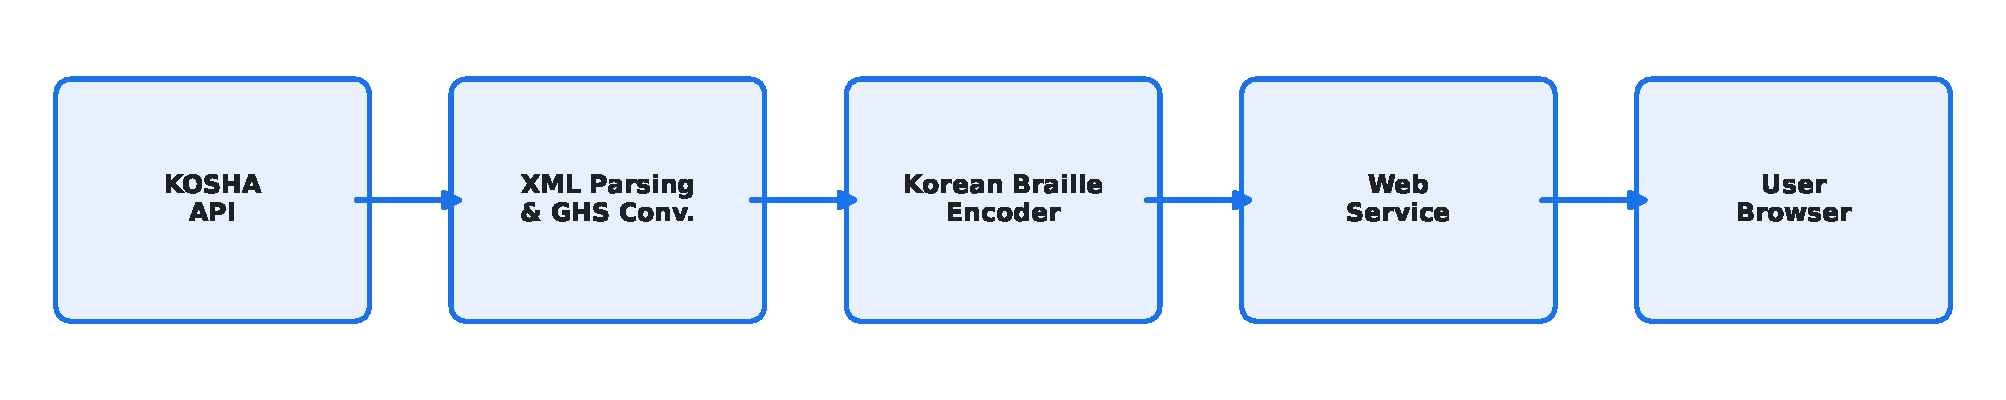
\includegraphics[width=\columnwidth]{fig_pipeline.pdf}
\caption{KOSHA-Braille 시스템 구조. MSDS 데이터를 KOSHA 공개 API로부터 수집하여 GHS 픽토그램 변환을 포함한 파싱·정제를 거쳐 2017년 한국 점자 규정에 따라 점자로 인코딩하고, 웹 인터페이스를 통해 제공한다.}
\label{fig:pipeline}
\end{figure}

\begin{enumerate}
\item \textbf{데이터 획득}: KOSHA MSDS 데이터를 공공데이터포털 REST API \cite{data_go_kr}로부터 받으며, 화학물질별로 표준화된 16개 MSDS 섹션을 XML 형식으로 제공한다.

\item \textbf{본문 추출}: XML 응답에서 한국어 본문을 파싱한다. GHS 픽토그램 참조(예: ``GHS06.gif'')는 서술적 한국어 본문(예: ``{급성독성}'')으로 해소하여, 점자 출력이 읽을 수 없는 파일명이 아니라 의미 있는 유해성 정보를 전달하도록 한다.

\item \textbf{점자 인코딩}: 한국어 본문을 2017년 한국 점자 규정에 따라 유니코드 점자(U+2800--U+28FF)로 변환한다.

\item \textbf{전달}: FastAPI 백엔드가 인코딩된 콘텐츠를 REST API로 제공하며, 참조 단일 페이지 프런트엔드는 검색과 시각/점자 병렬 보기를 제공한다. 다운로드는 점자 프린터용 BRF와 유니코드 \texttt{.txt} 형식으로 지원된다.
\end{enumerate}

\subsection{한국 점자 인코딩}

인코딩 과정은 결정론적이며 손실이 없다. 각 한글 음절은 유니코드 산술 연산으로 초성, 중성, 종성으로 분해되며, 각각이 고정된 점형에 대응한다.

인코더는 다음 네 가지 문자 유형을 적절한 점자 표시 부호와 함께 처리한다.

\begin{itemize}
\item \textbf{한글}: 점자 점형으로 직접 분해(별도 부호 불필요).
\item \textbf{숫자}: 수표(점 3-4-5-6) 뒤에 숫자 점형 표기.
\item \textbf{로마자}: 로마자 표시(점 3-5-6) 뒤에 알파벳 점형, 대문자에는 대문자 표시(점 6) 추가.
\item \textbf{문장 부호}: 한국 점자 문장 부호 패턴으로 직접 매핑.
\end{itemize}

된소리(겹자음)는 점 6 접두 셀 다음에 본 자음 점형을 배치한다. 복모음과 복종성은 다중 셀 시퀀스를 사용한다.

\ref{tab:cho}, \ref{tab:jung}, \ref{tab:jong}표는 각각 초성, 중성, 종성의 전체 대응을 보여 준다. \ref{fig:encoding_example}그림은 두 가지 대표 MSDS 토큰(``메탄올'', ``인화성'')에 대한 전체 변환 경로를 예시한다.

\begin{figure}[H]
\centering
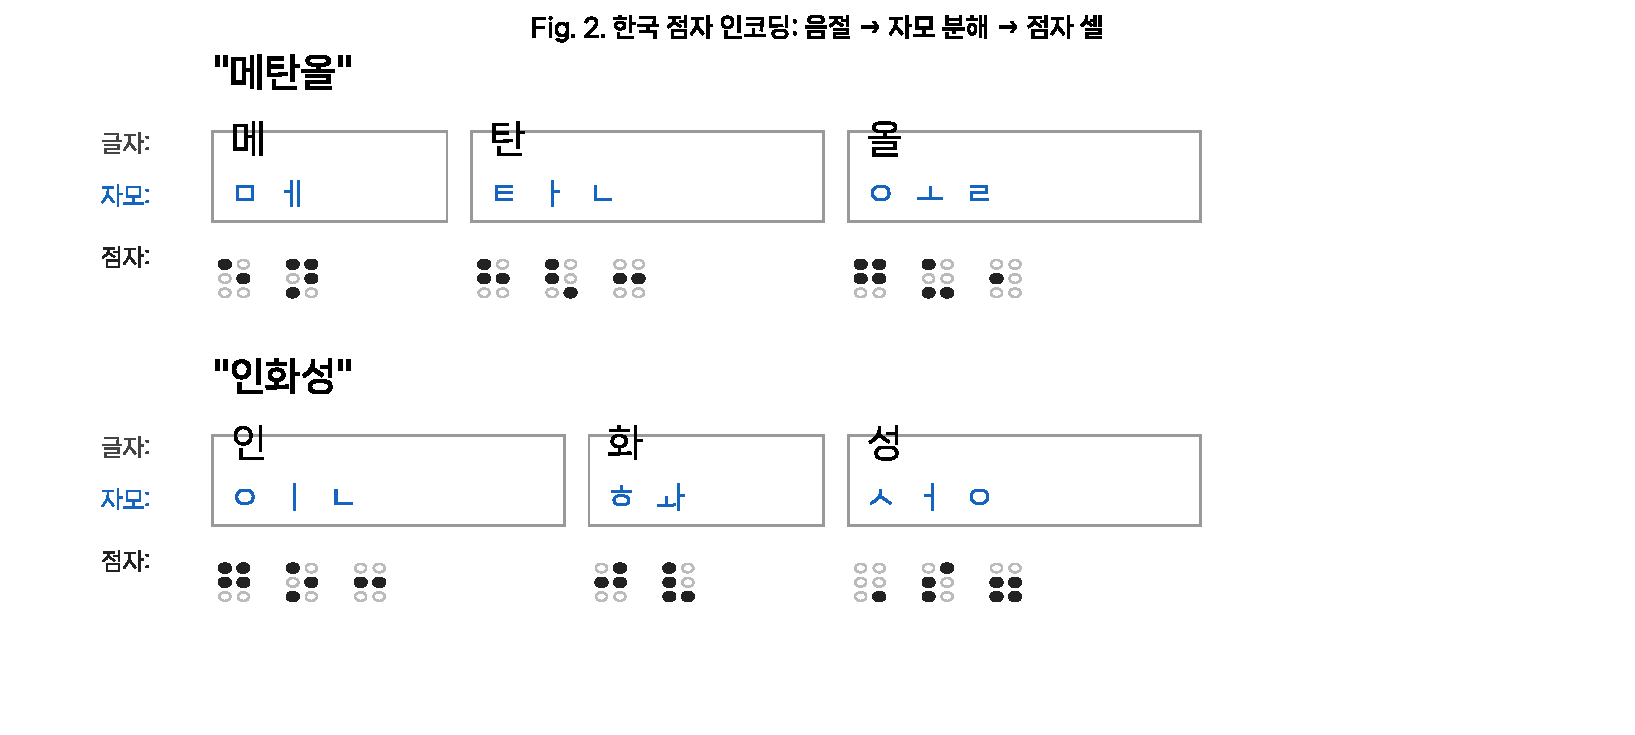
\includegraphics[width=\columnwidth]{fig_encoding_example_ko.pdf}
\caption{인코딩 예시: 각 한글 음절은 초성·중성·종성 자모(파랑)로 분해되고, 각 자모는 하나의 한국 점자 셀로 출력된다. 빈 원은 2$\times$3 점자 셀에서 사용되지 않은 점 위치를 나타낸다.}
\label{fig:encoding_example}
\end{figure}

\begin{table}[h]
\centering
\caption{초성 점자 점형}
\label{tab:cho}
\begin{tabular}{cccc}
\toprule
자음 & 점 & 자음 & 점 \\
\midrule
{ㄱ} & 4 & {ㅅ} & 6 \\
{ㄴ} & 1-4 & {ㅇ} & 1-2-4-5 \\
{ㄷ} & 2-4 & {ㅈ} & 4-6 \\
{ㄹ} & 5 & {ㅊ} & 5-6 \\
{ㅁ} & 1-5 & {ㅋ} & 1-2-4 \\
{ㅂ} & 4-5 & {ㅌ} & 1-2-5 \\
& & {ㅍ} & 1-4-5 \\
& & {ㅎ} & 2-4-5 \\
\bottomrule
\end{tabular}
\end{table}

\begin{table}[h]
\centering
\caption{중성 점자 점형}
\label{tab:jung}
\begin{tabular}{cccc}
\toprule
모음 & 점 & 모음 & 점 \\
\midrule
{ㅏ} & 1-2-6 & {ㅗ} & 1-3-6 \\
{ㅐ} & 1-2-3-5 & {ㅛ} & 3-4-6 \\
{ㅑ} & 3-4-5 & {ㅜ} & 1-3-4 \\
{ㅓ} & 2-3-4 & {ㅠ} & 1-4-6 \\
{ㅔ} & 1-3-4-5 & {ㅡ} & 2-4-6 \\
{ㅕ} & 1-5-6 & {ㅢ} & 2-4-5-6 \\
{ㅖ} & 3-4 & {ㅣ} & 1-3-5 \\
\bottomrule
\end{tabular}
\end{table}

\begin{table}[h]
\centering
\caption{종성 점자 점형}
\label{tab:jong}
\begin{tabular}{cccc}
\toprule
자음 & 점 & 자음 & 점 \\
\midrule
{ㄱ} & 1 & {ㅇ} & 2-3-5-6 \\
{ㄴ} & 2-5 & {ㅈ} & 1-3 \\
{ㄷ} & 3-5 & {ㅊ} & 2-3 \\
{ㄹ} & 2 & {ㅋ} & 2-3-5 \\
{ㅁ} & 2-6 & {ㅌ} & 2-3-6 \\
{ㅂ} & 1-2 & {ㅍ} & 2-5-6 \\
{ㅅ} & 3 & {ㅎ} & 3-5-6 \\
\bottomrule
\end{tabular}
\end{table}

\section{데이터셋 기술}
\label{sec:dataset}

\subsection{원본 데이터}

KOSHA-Braille 데이터셋은 안전보건공단(KOSHA)의 물질안전보건자료 데이터베이스에서 도출되며, 공공데이터포털 API \cite{data_go_kr}를 통해 일 호출 한도 10만 회의 인증 운영 계정으로 접근한다.

\subsection{데이터셋 통계}

\ref{tab:stats}표는 공개된 JSONL 산출물로부터 직접 재계산한 데이터셋 특성을 요약한다. \ref{fig:stats}그림은 문자 분포와 화학물질당 본문 길이의 경험적 분포를, \ref{fig:section_coverage}그림은 섹션별 커버리지와 평균 길이를 보여 준다.

\begin{figure}[H]
\centering
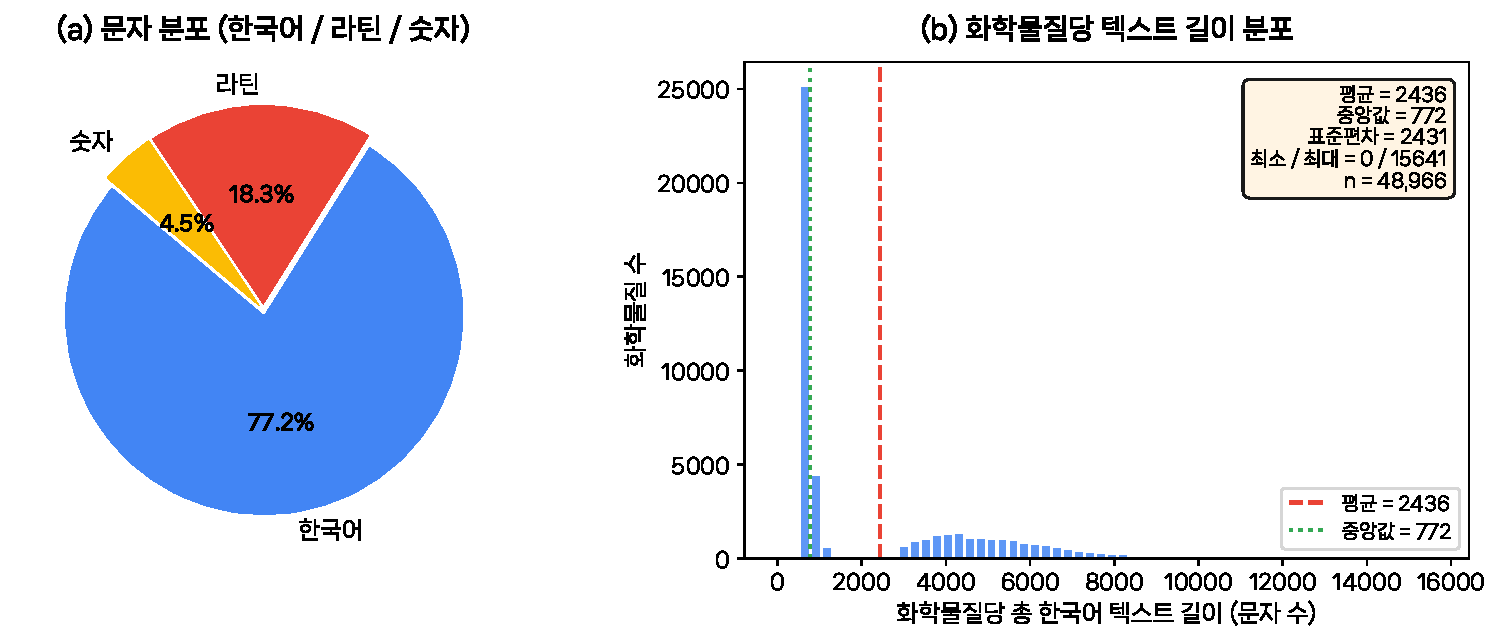
\includegraphics[width=\columnwidth]{fig_dataset_stats_ko.pdf}
\caption{공개 JSONL 기준 데이터셋 특성($n=48{,}966$ 화학물질). (왼쪽) 문자 유형 분포. (오른쪽) 화학물질당 총 한국어 본문 길이 히스토그램. 양봉 형태는 16개 섹션을 모두 갖춘 화학물질과 KOSHA 기록에 실질 본문이 일부 섹션에만 들어 있는 화학물질의 혼재를 반영한다.}
\label{fig:stats}
\end{figure}

\begin{table}[H]
\centering
\caption{KOSHA-Braille 데이터셋 통계}
\label{tab:stats}
\begin{tabular}{lr}
\toprule
지표 & 값 \\
\midrule
화학물질 수 & 48,966 \\
원본 DB 섹션 행 수 & 769,897 \\
공개 비어 있지 않은 섹션 수 & 401,272 \\
화학물질당 평균 비어 있지 않은 섹션 & 8.2 (전체 스키마: 16) \\
한국어 본문(총) & 1억 1{,}930만 문자 \\
한국 점자(총) & 2억 3{,}230만 셀 \\
점자:본문 평균 비율 & 1.95 \\
\midrule
\multicolumn{2}{l}{\emph{화학물질당 한국어 본문 길이}} \\
\quad 평균 & 2{,}436 문자 \\
\quad 중앙값 & 772 문자 \\
\quad 표준편차 & 2{,}431 문자 \\
\quad 최소 / 최대 & 0 / 15{,}641 문자 \\
\midrule
\multicolumn{2}{l}{\emph{문자 유형(분류된 문자 기준)}} \\
\quad 한국어(한글) & 77.2\% \\
\quad 라틴어        & 18.3\% \\
\quad 숫자          & 4.5\% \\
\bottomrule
\end{tabular}
\end{table}

\begin{figure}[H]
\centering
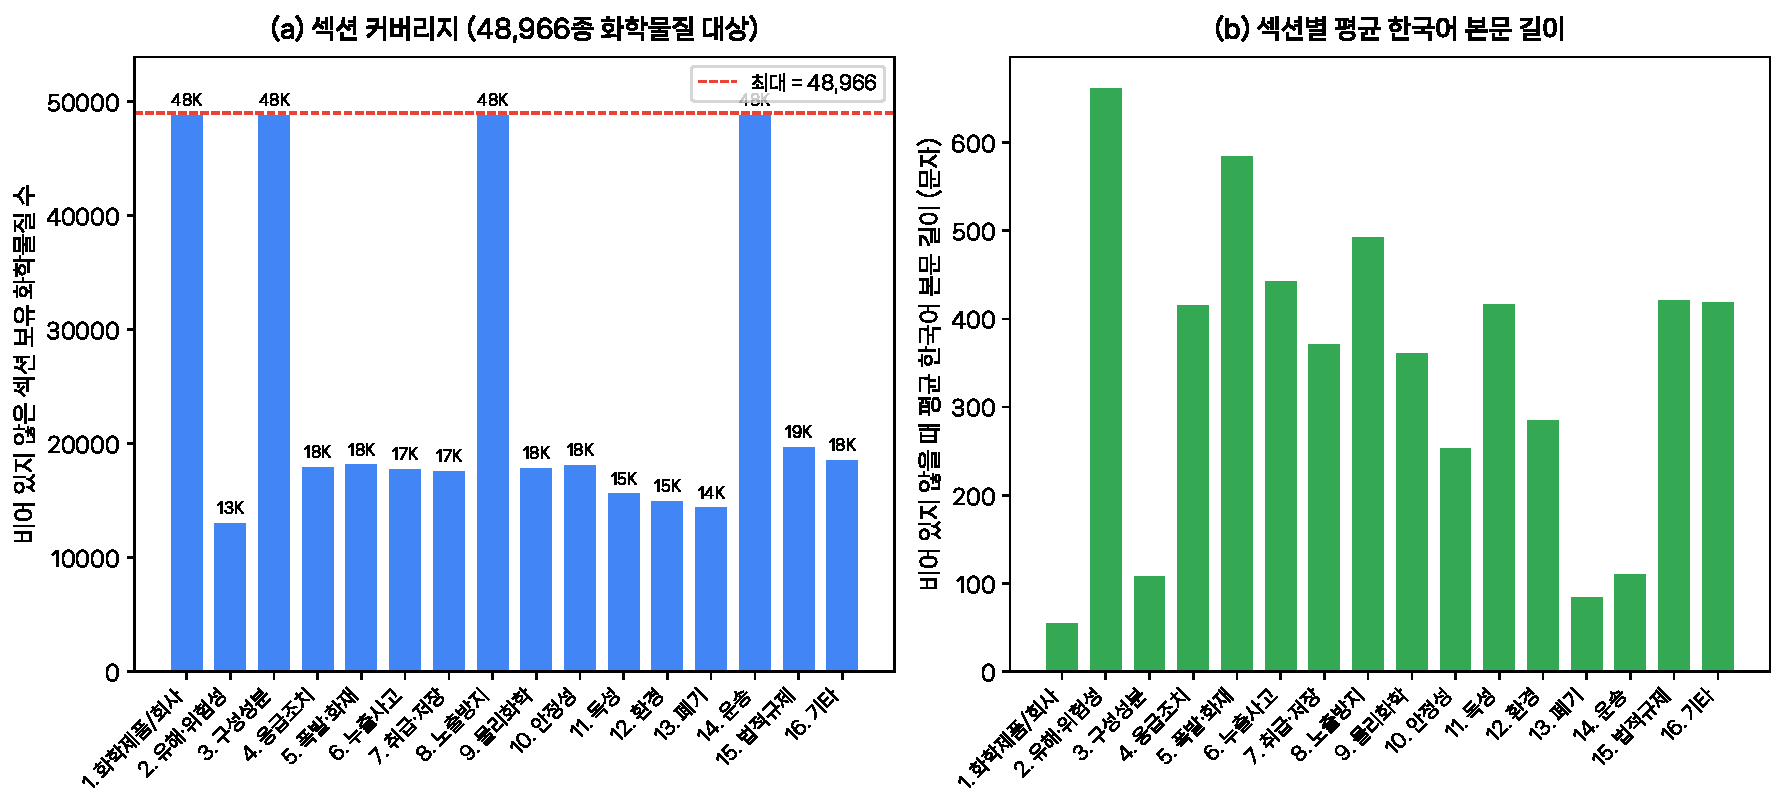
\includegraphics[width=\columnwidth]{fig_section_coverage_ko.pdf}
\caption{KOSHA가 정의한 16개 MSDS 섹션에 대한 공개 데이터셋의 섹션별 커버리지. (a) 각 섹션에 비어 있지 않은 본문을 가진 화학물질 수. 1번(화학제품/회사 정보), 3번(구성성분), 8번(노출방지), 14번(운송)은 사실상 모든 화학물질에 채워져 있고, 규제·물리화학 상세 섹션은 원본 KOSHA 기록이 자료 없음 표시가 아닌 실내용을 담은 경우에만 채워져 있다. (b) 각 섹션의 평균 한국어 본문 길이(섹션이 비어 있지 않은 경우 조건부).}
\label{fig:section_coverage}
\end{figure}

\subsection{GHS 픽토그램 변환}

원본 MSDS 데이터는 GHS 유해성 픽토그램을 이미지 파일명(예: ``GHS06.gif'')으로 참조하며, 이는 점자에서는 무의미하다. 본 시스템은 이를 \ref{tab:ghs}표와 같이 서술적 한국어 본문으로 해소한다. 데이터베이스에 출현하는 147개 고유 H/P 문구 코드(H 문구 63종, P 문구 84종)가 모두 해소되어 인코딩된다.

\begin{table}[h]
\centering
\caption{GHS 픽토그램 한국어 본문 변환}
\label{tab:ghs}
\begin{tabular}{lll}
\toprule
코드 & 영어 & 한국어 \\
\midrule
GHS01 & Explosive & {폭발성} \\
GHS02 & Flammable & {인화성} \\
GHS03 & Oxidizing & {산화성} \\
GHS04 & Compressed gas & {고압가스} \\
GHS05 & Corrosive & {부식성} \\
GHS06 & Acute toxicity & {급성독성} \\
GHS07 & Irritant & {경고} \\
GHS08 & Health hazard & {건강유해성} \\
GHS09 & Environmental & {수생환경유해성} \\
\bottomrule
\end{tabular}
\end{table}

\subsection{공개}

전체 코퍼스는 HuggingFace 호환 스키마의 단일 JSONL 파일(943~MB)로 공개되며, 출처, 라이선스, 섹션 스키마, 사용 의도를 명시한 데이터셋 카드를 포함한다. 인코더, 디코더, 참조 서비스는 오픈소스 코드로 공개된다.

\section{검증}
\label{sec:validation}

\subsection{결정론적 정확성}

2017년 규정 하에서의 한국 점자 인코딩은 결정론적이고 규칙으로 정의된 변환이다. 각 한글 음절은 모호함 없이 초성·중성·선택적 종성으로 분해되며 각각이 고정 점형에 대응한다. 따라서 정확성은 매핑표와 그 적용을 검증하는 문제로 환원되며, 출력별 인간 점역사 평가를 요구하지 않는다. 표본 기반 인간 검증이 전수 커버리지를 달성할 수 없는 인프라 규모의 코퍼스에서 이는 중요한 성질이다.

\subsection{교차 참조 검증}

인코더는 독립적으로 개발된 오픈소스 한국 점자 변환기 \cite{hangul_braille_converter}와의 비교를 통해 검증되었다. \ref{tab:validation}표가 그 결과를 보여 준다.

\begin{table}[h]
\centering
\caption{교차 참조 검증 결과}
\label{tab:validation}
\begin{tabular}{lrr}
\toprule
검증 대상 & 표본 수 & 일치율 \\
\midrule
기본 한글 음절 & 41 & 100\% \\
한국어 골든 문장 & 45 & 100\% \\
MSDS 화학물질명 & 356 & 100\% \\
\midrule
\textbf{합계} & \textbf{442} & \textbf{100\%} \\
\bottomrule
\end{tabular}
\end{table}

\subsection{인코딩 속성}

\begin{itemize}
\item \textbf{결정론적}: 동일 입력은 항상 동일 출력을 생성한다.
\item \textbf{단사(injective)}: 서로 다른 한글 음절은 서로 다른 한국 점자 문자열을 생성한다(한글 유니코드 분해를 통한 알고리즘적 검증, 그리고 442개 교차 참조 입력 전반에서 확인).
\item \textbf{표준 준수}: 모든 점형이 2017년 한국 점자 규정 \cite{ko_braille_2017}과 일치한다.
\end{itemize}

\subsection{검증의 범위}

본 검증은 인코딩 매핑이 참조 구현 및 공포된 규정과 일치함을 확립한다. 보고된 한국어 라운드트립 수치는 명시적 한국어 디스패치 하의 디코더 경로 검증으로 해석되며, 인코더의 정확성을 부정하는 증거로 사용되지 않는다. 현재 한국어 디코더가 혼합 표기·문장 부호·괄호·인용·숫자열에 대해 강화된 상태에서, 공개 골든 셋은 45/45로 라운드트립하며, 지속 스트레스 코퍼스는 27개 혼합 형식 사례에서 0건의 실패를, 동봉 샘플 DB에 대한 반복 무작위 표본 점검에서도 0건의 실패를 보고한다. 본 연구는 시각장애 독자를 대상으로 한 읽기 이해 사용자 연구를 포함하지 않으며, 이를 필수 후속 작업으로 명시한다. 한국 2종(축약) 점자는 구현되지 않았다. 본 코퍼스는 전반에 걸쳐 1종 점자이다.

\section{참조 배포}
\label{sec:webservice}

\subsection{구조}

웹 서비스는 단일 페이지 HTML/JavaScript 프런트엔드를 갖춘 FastAPI(Python)로 구축되어 있다. SQLite가 사전 수집된 MSDS XML을 저장하며, 점자 변환은 요청 시 수행되어 화학물질당 일반적으로 500\,ms 이하로 응답한다.

\subsection{API 엔드포인트}

\begin{itemize}
\item \texttt{GET /api/stats} -- 코퍼스 통계
\item \texttt{GET /api/chemicals?search=} -- 한국어 명칭 또는 CAS 번호로 검색
\item \texttt{GET /api/chemicals/\{id\}} -- 전체 MSDS 본문
\item \texttt{GET /api/chemicals/\{id\}/braille} -- 한국 점자가 포함된 MSDS
\item \texttt{GET /api/chemicals/\{id\}/braille.txt} -- 유니코드 점자 다운로드
\item \texttt{GET /api/chemicals/\{id\}/braille.brf} -- BRF(점자 프린터) 다운로드
\item \texttt{POST /api/convert} -- 즉석 한국어$\rightarrow$점자 변환
\end{itemize}

\subsection{사용자 인터페이스와 소비 경로}

시각적 좌우 병렬 뷰(\ref{fig:webui}그림)는, 점자 생산이 존재하며 한국어 원문과 일관됨을 확인해야 하는 비장애 이해관계자(규제기관, 조달 담당자, 감사관)를 위한 제시 표면이다. 점자 독자에게 기능적으로 중요한 출력은 다운로드 가능한 BRF와 유니코드 파일이다. 이들은 (1) 로컬 기기나 휴대전화에서 USB·블루투스로 연결한 점자 디스플레이, (2) 하드카피 생성을 위한 점자 프린터, (3) 데스크탑·모바일의 접근 가능한 읽기 소프트웨어로 직접 투입된다. 본 배포는 명시적으로 제품이 아닌 참조 구현이며, 그 목적은 코퍼스가 기존 보조 하드웨어·소프트웨어로 종단 간 소비 가능함을 시연하는 데 있다.

\begin{figure}[H]
\centering
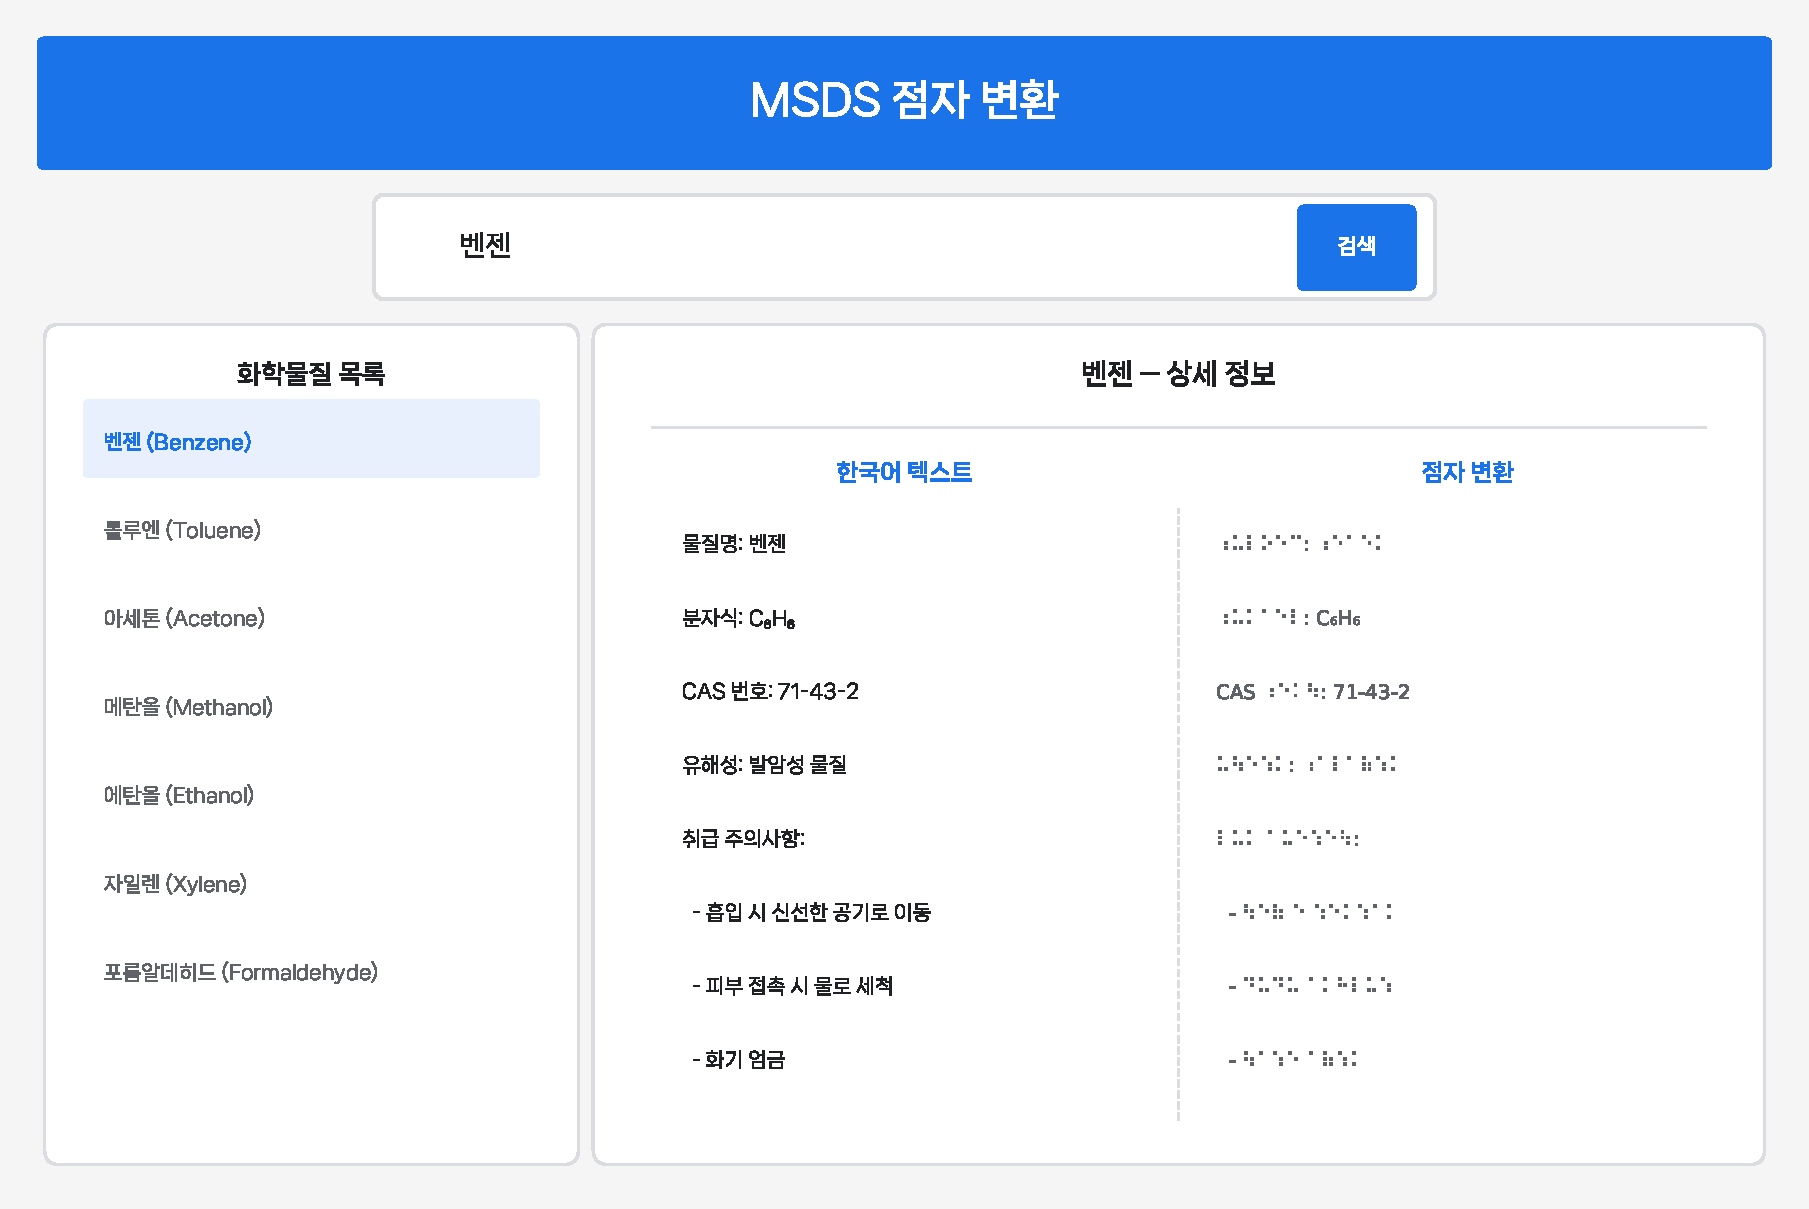
\includegraphics[width=\columnwidth]{fig_webui.pdf}
\caption{화학물질 검색(상단), 결과 목록(좌측), 한국어 본문과 점자의 좌우 병렬 표시(우측)를 보여 주는 웹 서비스 사용자 인터페이스.}
\label{fig:webui}
\end{figure}

\section{확장성}
\label{sec:extensibility}

본 논문의 중심 주장 가운데 하나는 KOSHA-Braille가 종착점이 아니라 템플릿이라는 것이다. 우리는 이 주장을 현재 릴리스로 입증된 \emph{검증된 확장성}(validated extensibility)과 아키텍처적으로 가능하지만 코퍼스 규모로는 아직 수행되지 않은 \emph{전망적 확장성}(prospective extensibility)으로 분리하여, 증거와 전망의 경계를 명시한다.

\subsection{검증된 확장성(현재 릴리스)}

다음 확장들은 현재 릴리스로 실제 수행되었으며 따라서 전망이 아닌 증거이다.

\begin{itemize}
\item \textbf{한국 MSDS 체제 전체}: 48{,}966종 화학물질, 401{,}272개 비어 있지 않은 섹션, 수집·GHS 해소·점자 인코딩·BRF/유니코드 전달·참조 웹 서비스에 이르는 종단 간 수행. 이는 본 파이프라인의 검증된 적용 영역이다.
\item \textbf{식품 알레르겐 표시}: 한국 식품표시 규정상 19개 범주를 인코딩·내보내기 완료(\texttt{data/domain\_expansion/food\_allergens\_braille.jsonl}).
\item \textbf{응급조치·산업보건 프로토콜}(KISCHEM): 원본 DB는 7{,}189건의 기록을 담고 있으며, 영역 확장 시연으로 100건 점자 내보내기를 동봉한다(\texttt{kischem\_firstaid\_braille.jsonl}). 종단 간 경로는 소규모에서 수행되었고, 전체 내보내기는 운영상 가능하나 본 릴리스에는 포함되지 않는다.
\item \textbf{CAS 키 기반 교차 참조}: KOSHA MSDS 기록에 연결된 13{,}445종의 고유 CAS 번호와 프로젝트에 동봉된 74{,}494건의 CAS$\rightarrow$PubChem~CID 매핑은 한 번 인코딩되어 재변환 없이 재사용되며, 이는 PubChem, ECHA, EPA, OSHA 등록부로의 언어 독립적 가교를 시연한다.
\end{itemize}

\subsection{전망적 확장성(아키텍처적, 아직 수행되지 않음)}

다음 확장들은 아키텍처적으로 지원되지만 본 릴리스에서 수행되지는 않았다. 리뷰어가 완료된 작업으로 오해하지 않도록 전망으로 명시한다.

\begin{itemize}
\item \textbf{의약품 표시와 첨부문서 전체 점자}(한국 식품의약품안전처): 규제된 점자에 관한 가장 좁은 국제 선례(EU 의약품 포장 \cite{eu_braille})는 제품명에만 적용되며, 표시 전문 점자는 아키텍처적 직접 확장이지만 본 코퍼스에는 포함되지 않는다.
\item \textbf{K-REACH 화학물질 등록 신고}: 원본 DB는 47{,}344종 등록 물질을 담고 있다. 파이프라인은 이를 동일 인코더로 처리하는 병렬 수집 경로로 다룰 수 있으나, K-REACH 점자 내보내기는 본 릴리스에 포함되지 않는다.
\item \textbf{법령·행정 결정}으로서 산업안전·화학 규제 관련 문서: 동일 템플릿이 적용 가능하며, 법령 전용 수집기와 동일 점자 인코더만 추가로 요구된다.
\item \textbf{국가 간 SDS}(미국 OSHA HazCom, EU CLP/REACH, 일본 J-CHECK): ``구조화된 규제 원문 $\rightarrow$ 언어별 점자 코퍼스'' 패턴이 적용되며, 적용에는 각 체제별 수집과 점자 규정의 교체가 요구된다.
\end{itemize}

\subsection{언어 확장성}

언어 의존적 구성 요소는 인코더 하나뿐이다. 다른 점자 규정---일본(2001), 중국(만다린 점자), 영어 UEB, EU 각국 규정---에 대해 규칙 테이블을 교체하면 파이프라인의 나머지가 보존된다. 본 릴리스 내에서 이는 아키텍처적이다(현재 인코더는 한국어 전용). 교체는 기계적이지만 두 번째 규정에 대해 실제로 수행된 바는 없다.

\subsection{소비 형식 확장성}

현재 릴리스는 유니코드 점자(U+2800--U+28FF)와 BRF를 제공한다. 단기 확장 후보로는 점자 양각·열성형 표시를 위한 촉각 SVG, GHS 픽토그램의 촉각 그래픽 파생물, CAS·ICSC 식별자를 연결하는 JSON-LD 주석이 있다. 이들은 릴리스 구성 요소가 아니라 로드맵 항목으로 명시한다.

\subsection{정책 확장성}

본 코퍼스는 정책 제안의 구체 근거가 되는 산출물이다. KOSHA의 공식 접근 가능 형식 채택, 고용노동부 조달 표준에의 편입, 그리고 점자 프린터 출력이 가능한 기업 환경·보건·안전(EHS) 시스템과의 통합이 그 예이다.

\section{논의}
\label{sec:discussion}

\subsection{적절한 평가 기준}

우리는 KOSHA-Braille가 사용 채택량으로 평가되지 않음을 명시한다. 인프라급 접근성 산출물에 적절한 기준은 다음과 같다.

\begin{enumerate}
\item 비장애 독자의 대응물과의 커버리지 동등성(본 사례에서는 KOSHA MSDS 기록의 100\%).
\item 표준 준수(\ref{sec:validation}장에서 검증).
\item 결정론성과 재현성.
\item 가용성(자유 접근. 기관·페이월 제한 없음).
\item 확장성(\ref{sec:extensibility}장).
\end{enumerate}

이 기준에 따르면 현재 시스템은 실질적 진보이다. 한국 화학 안전 점자에 관한 이전의 최고 기술 수준은 부재였다.

\subsection{발생 빈도는 낮으나 결과가 중대한 접근성}

화학 안전은 더 넓은 부류의 접근성 대상의 한 사례이다. 그 부류는 기술·규제 정보 영역으로, 관측된 시각장애 사용자 수는 작지만 접근이 부재할 때의 결과가 중대한 영역이다. 이 부류의 다른 구성원에는 법령과 판례, 의료 가이드라인, 표준 문서, 행정 참고 자료 등이 있다. 이러한 영역에 점자 인프라를 구축하는 데 대한 경제적 반론은 각 사례에서 동일하며, 동일하게 반박된다. 관측된 사용자 수는 인프라의 함수이지 인프라에 관한 독립적 사실이 아니다.

\subsection{주장의 범위: 무엇이 검증되었고 무엇이 검증되지 않았는가}
\label{sec:scope-of-claims}

리뷰어가 경계를 추론할 필요가 없도록 검증 주장을 두 층위로 분리한다.

\paragraph{검증된 것.}
(a) 인코더는 2017년 한국 점자 규정의 결정론적 구현이다. (b) 기본 음절, 골든 문장, 실 MSDS 화학물질명에 걸친 442건의 교차 참조 사례에서 독립적으로 개발된 오픈소스 한국 점자 변환기와 100\% 일치한다. (c) 공개 디코더 경로는 공개 45문장 한국어 골든 셋을 45/45로 라운드트립하며 27건 디코더 스트레스 코퍼스에서 0건의 실패를 보고한다. (d) 규제 기록 커버리지가 완전하다. KOSHA MSDS 데이터베이스에 존재하는 모든 화학물질이 공개 코퍼스에 포함된다.

\paragraph{아직 검증되지 않은 것.}
(a) 시각장애 독자에 의한 읽기 이해. (b) 현장 조건에서 점자 디스플레이와 점자 프린터를 통한 BRF·유니코드 출력의 주관적 사용성. (c) GHS 픽토그램--한국어 본문 해소가 점자 독자의 유해성 인식에 충분한지(대안적 촉각 그래픽이나 청각 신호와의 비교).

\paragraph{본 제출이 (a)--(c) 없이 성립하는 이유.}
연기된 항목들은 \emph{독자와 산출물의 상호작용}에 대한 평가이다. 반면 검증된 항목들은 \emph{산출물이 존재하며, 표준에 부합하고, 비장애 독자 버전과 커버리지가 동등하며, 표준 보조 하드웨어로 종단 간 소비 가능함}을 확립한다. 전자의 범주는 후자를 전제한다. 현 단계에서 통계적 검정력이 부족한 사용자 연구를 보고하는 것은 오히려 기여를 약화시키며, 인프라 릴리스를 사용성 주장으로 오해하게 만든다. 따라서 우리는 인프라를 지금 공개하고, 경계를 문서화하며, 사용자 평가는 별도로 적절히 검정력 있게 수행될 후속 연구로 명시한다.

\subsection{알려진 한계}

\begin{enumerate}
\item \textbf{읽기 이해 사용자 연구 부재}(\ref{sec:scope-of-claims}절에서 별도로 다룸).
\item \textbf{1종 점자만 지원}: 한국 2종(축약) 점자는 문서 길이를 단축하지만 맥락 의존적 축약 결정이 도입되어 현 단계의 엄격한 결정론과 양립하지 않는다.
\item \textbf{초성/종성 경계에서의 디코더 모호성}: 한국 점자에 본래 내재한 문제이지만, 현재 공개된 한국어 디코더 경로는 공개 골든 셋을 45/45로 라운드트립한다. 잔여 위험은 따라서 현재 벤치마크 집합이 아닌 미관측 실세계 가장자리 사례에 집중된다.
\item \textbf{번역된 원문에서의 영역 용어}: 사용된 경우의 기계 번역 MSDS 콘텐츠가 도메인 용어 오류를 포함할 수 있으며, 이는 점자로 전파될 수 있다.
\end{enumerate}

\subsection{유지보수와 갱신 모델}
\label{sec:maintenance}

상류의 KOSHA MSDS 데이터베이스 자체가 갱신되므로, 한 번 공개하고 더 이상 갱신되지 않는 접근성 코퍼스는 시간이 지남에 따라 의미를 잃는다. 우리는 따라서 본 릴리스를 유지 가능한 갱신 모델에 묶는다. (i) 수집 계층은 공공데이터포털 API 엔드포인트로 매개변수화되어 있고 라이브 데이터 소스에 대해 멱등적으로(idempotently) 실행되므로, 갱신된 상류에 대한 재추출이 단일 명령 연산이다. (ii) 인코더, 디코더, GHS 해소 계층은 결정론적이며 폐쇄형 의존성 없이 자체 포함된 Python으로 작성되어, 재현에는 Python과 공개 저장소에 명시된 소수의 의존성만 필요하다. (iii) HuggingFace 데이터셋 카드와 GitHub 저장소가 버전 관리되므로, 하위 소비자는 특정 코퍼스 스냅샷에 고정(pin) 가능하다. (iv) 보조 패키지에 동봉된 검증 스크립트는 공개 JSONL만으로 본 논문의 모든 수치적 주장을 재생성하므로, 제3자 재실행자가 저자와의 조율 없이 향후 재추출을 검증할 수 있다. 단독 저자 위험은 실재하며 인정한다. 위의 완화 조치들은 단독 저자 릴리스가 사용 가능한 구조적 수단이다.

\section{결론}
\label{sec:conclusion}

본 논문은 한국 화학 안전 정보에 대한 접근성 인프라로서 KOSHA-Braille를 제시하였다. 769{,}897행의 원본 섹션 데이터베이스에서 401{,}272개의 비어 있지 않은 섹션을 공개한 48{,}966종 화학물질 규모, 총 2억 3{,}230만 점자 셀의 코퍼스가 결정론적·표준 준수 인코더로 생산되어 참조 배포와 함께 공개되었다. 우리는 이러한 작업에 적절한 프레이밍이 사용량 주도 서비스 전달이 아닌, UN 장애인권리협약 제9조 \cite{crpd} 및 한국 장애인차별금지법 제21조 \cite{kdpa}에 따른 인프라 제공임을 논증하였다. 본 시스템이 영역(의약품 표시, 식품 알레르겐, 응급조치 프로토콜, K-REACH 신고, 법령 본문), 언어(점자 인코더의 교체로), 규제 체제(미국 OSHA, EU CLP/REACH, 일본 J-CHECK)에 걸쳐 확장 가능하도록 만드는 아키텍처 속성은 \ref{sec:extensibility}장에서 다루었다.

이러한 종류의 작업에 대한 근거는 다음 달에 얼마나 많은 독자가 사용하는가에 있지 않다. 그 근거는 필요한 읽기 인프라가 부재할 때 직역에 진입할 수 없는 사람---국회에서 질문할 수 없는 사람, 법정에서 주장을 펼칠 수 없는 사람, 보도국에서 취재를 제기할 수 없는 사람---에게 있다. 후속 작업으로는 시각장애 독자를 대상으로 한 읽기 이해 사용자 연구, 한국 2종(축약) 점자 지원, GHS 픽토그램의 촉각 그래픽 처리, 그리고 관련 규제기관의 공식 접근 가능 형식으로의 채택이 있다.

본 논문이 전반에 걸쳐 견지하는 범위 경계를 마지막으로 강조한다. 본 논문의 기여는 접근성 인프라의 설계·검증·공개 릴리스이지, 최종 사용자 읽기 성능에 관한 주장이 아니다. 본 릴리스 이후의 인프라 유지보수는 \ref{sec:maintenance}절에 기술된 모델(라이브 KOSHA 엔드포인트에 대한 멱등 수집, 결정론적이고 자체 포함된 처리 계층, 버전 관리된 데이터셋 스냅샷, 제3자가 재현 가능한 검증 스크립트)에 묶이며, 이로써 본 릴리스가 일회성 산출물이 아닌 지속 가능한 인프라로 기능한다.

\section*{감사의 말}

저자는 물질안전보건자료 기록에 대한 공개 접근을 유지해 온 안전보건공단(KOSHA)과 공공데이터포털, 그리고 \ref{sec:validation}장에서 보고된 교차 참조 검증에 사용된 독립 오픈소스 한국 점자 변환기 \cite{hangul_braille_converter}의 메인테이너에게 감사를 표한다.

\section*{선언}

\subsection*{연구비}
본 연구는 외부 연구비를 받지 않았다. 계산 자원, 인프라, 데이터 포털 API 접근 비용은 저자가 직접 부담하였다.

\subsection*{이해상충}
저자는 재정적·비재정적 이해상충이 없음을 선언한다.

\subsection*{윤리와 동의}
본 연구는 인간 대상자, 동물 대상자, 개인식별정보를 포함하지 않는다. 원본 데이터는 공개된 규제 자료이다. 윤리 승인, 참여 동의, 발표 동의는 모두 해당 없음.

\subsection*{저자 기여}
단독 저자가 구상, 설계, 구현, 검증, 분석, 집필을 모두 수행하였다.

\section*{데이터와 코드 가용성}

데이터셋은 HuggingFace Datasets에 \texttt{Yuyongkim/inconvenience-msds}로 공개되어 있다 \cite{hf_dataset}. 인코더, 디코더, 파이프라인, 웹 서비스, 평가 하네스, 그리고 본 논문의 모든 수치적 주장을 생산하는 데 사용된 검증 스크립트는 GitHub의 \texttt{yuyongkim/inconvenience-msds}에 공개되어 있다 \cite{github_repo}. MSDS 원본 데이터는 공공데이터포털 \cite{data_go_kr}을 통해 공개적으로 접근 가능하다. 데이터셋 라이선스: CC BY~4.0; 코드 라이선스: MIT.

\begin{thebibliography}{20}

\bibitem{kosha_act}
Ministry of Employment and Labor, ``Occupational Safety and Health Act,'' Arts.~110--111, Republic of Korea, 2020.

\bibitem{crpd}
United Nations General Assembly, ``Convention on the Rights of Persons with Disabilities,'' Art.~9 (Accessibility), Resolution A/RES/61/106, adopted 13~December 2006, entered into force 3~May 2008.

\bibitem{kdpa}
Republic of Korea, ``Act on the Prohibition of Discrimination Against Persons with Disabilities and Remedy Against Infringement of Their Rights,'' Act No.~8341 (2007), latest amendment Act No.~10280; esp.\ Arts.~20--21 (Information Access). Official English translation: Korea Legal Research Institute, \url{https://elaw.klri.re.kr/}.

\bibitem{hamraie}
A.~Hamraie, \emph{Building Access: Universal Design and the Politics of Disability}. Minneapolis, MN: Univ.\ of Minnesota Press, 2017. ISBN 978-1-5179-0164-6.

\bibitem{curb_cut}
A.~G.~Blackwell, ``The curb-cut effect,'' \emph{Stanford Social Innovation Review}, vol.~15, no.~1, pp.~28--33, Winter 2017. DOI:~10.48558/YVMS-CC96.

\bibitem{bennett_keyes}
C.~L.~Bennett and O.~Keyes, ``What is the point of fairness? Disability, AI and the complexity of justice,'' \emph{ACM SIGACCESS Accessibility and Computing}, no.~125, art.~1, Mar.~2020. DOI:~10.1145/3386296.3386301.

\bibitem{wedler}
University of California, Davis, ``White House hails blind chemistry grad student as `Champion of Change','' UC~Davis News, July~2012; H.~Wedler, Ph.D.\ dissertation, Dept.\ of Chemistry, Univ.\ of California, Davis, 2016; Accessible Science, \url{https://accessiblescience.com/}.

\bibitem{nfb_legislators}
National Federation of the Blind, ``Blind Legislators and Public Officials,'' \url{https://nfb.org/}, accessed 2026.

\bibitem{disability_stats}
Korea Disabled People's Development Institute, ``2023 Disability Statistics Annual Report,'' Seoul, 2023.

\bibitem{eu_braille}
European Commission, ``Directive 2004/27/EC of the European Parliament and of the Council of 31~March 2004 amending Directive 2001/83/EC on the Community code relating to medicinal products for human use,'' Art.~56a, \emph{Official Journal of the European Union}, L~136, pp.~34--57, 30~April 2004.

\bibitem{liblouis}
liblouis developers, ``liblouis -- Open-source braille translator and back-translator,'' \url{https://github.com/liblouis/liblouis}, accessed 2026.

\bibitem{hangul_braille_converter}
hyonzin, ``hangul-braille-converter: Korean braille converter in Python,'' \url{https://github.com/hyonzin/hangul-braille-converter}, accessed 2026.

\bibitem{hanbraille}
delvier, ``hanbraille: Hangul Braille Converter,'' \url{https://github.com/delvier/hanbraille}, accessed 2026.

\bibitem{ghs}
United Nations Economic Commission for Europe, \emph{Globally Harmonized System of Classification and Labelling of Chemicals (GHS)}, 10th rev.~ed. New York and Geneva: United Nations, 2023.

\bibitem{ko_braille_2017}
Ministry of Culture, Sports and Tourism, ``Korean Braille Standards (한국 점자 규정),'' Notification No.~2017-15, Republic of Korea, 2017.

\bibitem{data_go_kr}
Korea Public Data Portal, ``KOSHA MSDS Open API,'' \url{https://www.data.go.kr/data/15001197/openapi.do}, accessed 2026.

\bibitem{kosha_system}
Korea Occupational Safety and Health Agency, ``Chemical Information System,'' \url{https://msds.kosha.or.kr/}, accessed 2026.

\bibitem{hf_dataset}
Y.~Kim, ``inconvenience-msds: Korean Chemical Safety MSDS in Braille,'' HuggingFace Datasets, 2026. \url{https://huggingface.co/datasets/Yuyongkim/inconvenience-msds}.

\bibitem{github_repo}
Y.~Kim, ``inconvenience-msds source code,'' GitHub, 2026. \url{https://github.com/yuyongkim/inconvenience-msds}.

\end{thebibliography}

\begin{IEEEbiography}[]{김유용}
화학공학 학사를 취득하였으며, 현재 위스콘신--매디슨 대학교에서 데이터 분석 석사 과정을 이수하고 있다. 12년간 석유화학·EPC 엔지니어로 근무한 산업 경력을 보유한다. 현재 연구는 화학공학·화학 안전 규제에 특화된 대형언어모델·검색 시스템, 기술·규제 정보 접근성 인프라, 그리고 한국 주식시장 정량 분석에 걸쳐 있다. 화학공학 분야 7-source 하이브리드 검색 시스템 ChemEng~AI, KOSHA 규정 기반 플랜트 엔지니어링 검증 플랫폼 EPC-KOSHA, 그리고 본 연구의 KOSHA-Braille 개발자이다.
\end{IEEEbiography}

\end{document}
